\section{Application Scenarios}
\label{sec:scenarios}
%
Our obstruction-free fish-eye lens can be used with different types of volumetric datasets. To illustrate this, we next present four such use-cases considering scalar density volumes coming from baggage inspection, 3D flow simulation, radiology, and air traffic management.

\subsection{Baggage inspection: An unusual blunt object}
\label{sec:baggage}
%
In most airports, security agents deal with volumetric data exploration during baggage inspections. While automatic systems are now able to detect densities of harmful substances such as C-4, TNT, and nitroglycerin, and event some prohibited articles such as classical firearms and knives, it remains difficult to identify unusual threats. In addition, baggage inspection faces four main concealment strategies\,\cite{7819413}:

\vspace{0.15cm}
\noindent\textbf{Superposition}: A threat (prohibited object) may be sheltered among dense materials. It is sometimes possible to see through such a `shield' using high penetration (enhanced X-ray power) or image processing (contrast improvement) techniques. However, such techniques are not universally available and also require fine-tuning various parameters, which slows down the inspection process.

\vspace{0.15cm}
\noindent\textbf{Location}: Depending on its location inside the luggage, a threat can be hard to detect. Objects located in the corners, edges, or in the luggage’s frame are very hard to spot.

\vspace{0.15cm}
\noindent\textbf{Dissociation}: One can conceal a threat by spreading its parts in the luggage, \emph{e.g}, by disassembling a weapon and scattering its parts.

\vspace{0.15cm}
\noindent\textbf{Lure}: A lure can be used to to hide the real threat. For instance, a minor threat like a small scissors c be clearly visible and catch the security agent's attention while a more important threat remains hidden.

Consider the baggage scan in \autoref{f:baggage_lens} with a volume size of 283x189x344 voxels. Automatic baggage inspection systems will not detect anything suspect on this scan. However, while visually exploring this baggage from different angles (\autoref{f:baggage_lens}a-c), it appears that an object is hidden between a set of mugs. A common solution to this type of issue in baggage inspection is to filter materials by density in order to show or hide subsets of the volume and reduce the occlusion. However, in this case, this solution does not work, as the suspect target has almost the same density as the surrounding mugs. Hence, removing the occludes will also remove the target (\autoref{f:baggage_lens}d-f). Using the obstruction-free fish-eye lens helps in this kind of situation. Clicking on the sharp detail visible in \autoref{f:baggage_lens}c first gathers rays so they pass through the low-density zone between the mugs (\autoref{f:baggage_lens}f)

The user has just to use this tool on the partially hidden target. Then, a transition inside the lens will start and smoothly provide the finale unobstructed view of the blunt object which is, in this case, a ceramic shuriken (\autoref{f:baggage_lens}e-g). However, this shows only a small part of the target. Scattering rays next fully reveals the target (\autoref{f:baggage_lens}h). The user can adjust the lens size to get a more detailed view of the target (\autoref{f:baggage_lens}i). Next, the user can locally turn the viewpoint around the target, as already shown in \autoref{f:rotation}. From these views, the controller decides that the target is a copy of a shuriken (Japanese ninja star weapon). However, since the object is very thick and blunt (see \autoref{f:rotation}), it is clearly not a threat.
\textcolor{red}{
Since we get this data-set from an airport, we had the opportunity to get a feedback from 3 baggage security practitioners. According to them, this tool is interesting as it can provide them a better perception of the items inside the baggage. But, this tool cannot be used for the carry-on luggage since they have a very small time-window to inspect one luggage (about 15s - 20s) in order to keep a smooth traffic flow (for economic reasons). Therefore, this tool is more suitable for checked baggage, where they have a longer time-window to inspect a suspect luggage (up to 3min). In fact, for the checked baggage, they only inspect suspect luggage thanks to an automatic system that identifies and displays them in the monitor of the practitioners. }

\subsection{Fluid flow: A deep-buried spherical vortex}
\label{sec:flow}
%
%
Flow visualization using streamlines has a long history in scientific visualization~\cite{brambilla2012illustrative,merzkirch2012flow}. When applied to 3D datasets, a key challenge is to balance the streamline density. Low values allow seeing inner regions in the data but can subsample (miss) important patterns. High values show more data but create too much occlusion. We next show how our lens can be used to discover interesting patterns in the second case, \emph{i.e.}, a 3D volume densely filled with streamlines. The dataset, introduced in\,\cite{griebel2004flow}, captures the simulation of water flow in a basin computed on a grid of 128x85x42 cells. A set of 4595 streamlines with 183K sample points is next traced by pseudo-random seeding over this vector field. We convert this set of 3D curves (polylines) to a scalar volume by using kernel density estimation (KDE)\,\cite{silverman1986density}. Similar techniques have been used to compute density maps of 2D trail-sets\,\cite{hurter2012graph,cubu,hurter2015image}. To increase computational speed, we compute the KDE in the frequency space and using GPU acceleration, following\,\cite{lhuillier2017ffteb}. The resulting volumes have a resolution of $500^3$ voxels and can be directly displayed using DVR (\autoref{f:stream_lens}). Note that, given the smoothing effect of KDE, streamlines appear now as finite-thickness tubes rather than pixel-thin curves.

For a first overview, we display the volume using standard DVR. After turning the viewpoint a bit, we notice a dense spherical item inside the dataset (\autoref{f:stream_lens}a). To see its shape better, we increase the opacity; however, this immediately increases occlusion so the item becomes invisible. Conversely, decreasing opacity to reduce occlusion makes the item almost transparent. Our lens solves the problem: In the initial view (\autoref{f:stream_lens}a), we point at the target and turn on the lens. This effectively pushes away the occluding stream bundles, and lets us see that our item is nearly perfectly spherical (\autoref{f:stream_lens}b). This is something we could not have assessed from \emph{any} viewpoint and with likely any opacity modulation using standard DVR. Our object is a set of densely-packed, low-speed, tightly-turning streamlines that create a ball-like vortex. Interestingly, this spherical vortex has not been discovered by any of the visualization techniques that we are aware of that used this same dataset\,\cite{telea_vis_99,griebel2004flow,ddh,lhuillier2017ffteb}. To make sure our target is spherical, we view it in the lens from different directions, by interactively changing the ray directions in the lens (\autoref{f:stream_lens}c). Finally, we can close the lens but keep the target magnified (\autoref{f:stream_lens}d).


\begin{figure*}[htb]
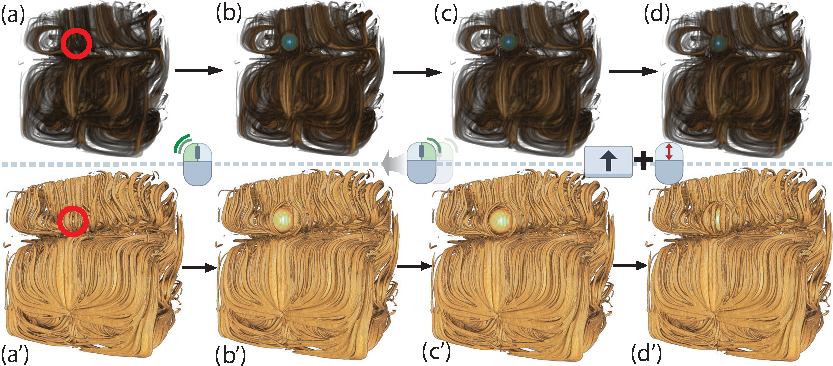
\includegraphics [width=\textwidth]{images/stream_lens.eps}
\caption{Flow volume exploration using two different opacity transfer functions (top and bottom rows). From the viewpoint (a), a small high-density spherical item appears between the streamlines. (b) The lens is applied at that location (double click). (c) The directions of rays inside the lens are changed to see the whole spherical target in the lens (right click + mouse drag change direction). (d) The lens is gradually closed while keeping the focus area magnified (shift + scroll).}
\label{f:stream_lens}
\end{figure*}

\subsection{Chest scan: A hard to see tumor}
%
In our third use-case, we consider a contrast chest CT scan (512x512x110 voxels) of an elderly patient having a sizeable (roughly 8 cm diameter) lung tumor. Typical examination of such data by the pulmonologist and radiologist in charge involves using slice-based views. In some of these views, the tumor is clearly visible (\autoref{f:slicer}a,c), though not in all of them (\autoref{f:slicer}b). Moreover, the exact tumor shape, morphology, and connection to the lung walls is not easy to assess. Using standard DVR makes the tumor partially visible (\autoref{f:slicer}d). However, occlusion from the rib cage and other tissues is still present. Using both TF presets and manually changing the TFs of the 3D Slicer tool\,\cite{slicer} used to construct the DVR could not help de-occluding the tumor without making (parts of) it transparent. This is also visible in the slice images in \autoref{f:slicer}a-c, where the gray values for the tumor and surrounding skin-and-muscle tissue on the rib cage are very similar. Hence, we cannot remove such occluding tissue by opacity TF manipulation without also removing the tumor.

\begin{figure}[htb]
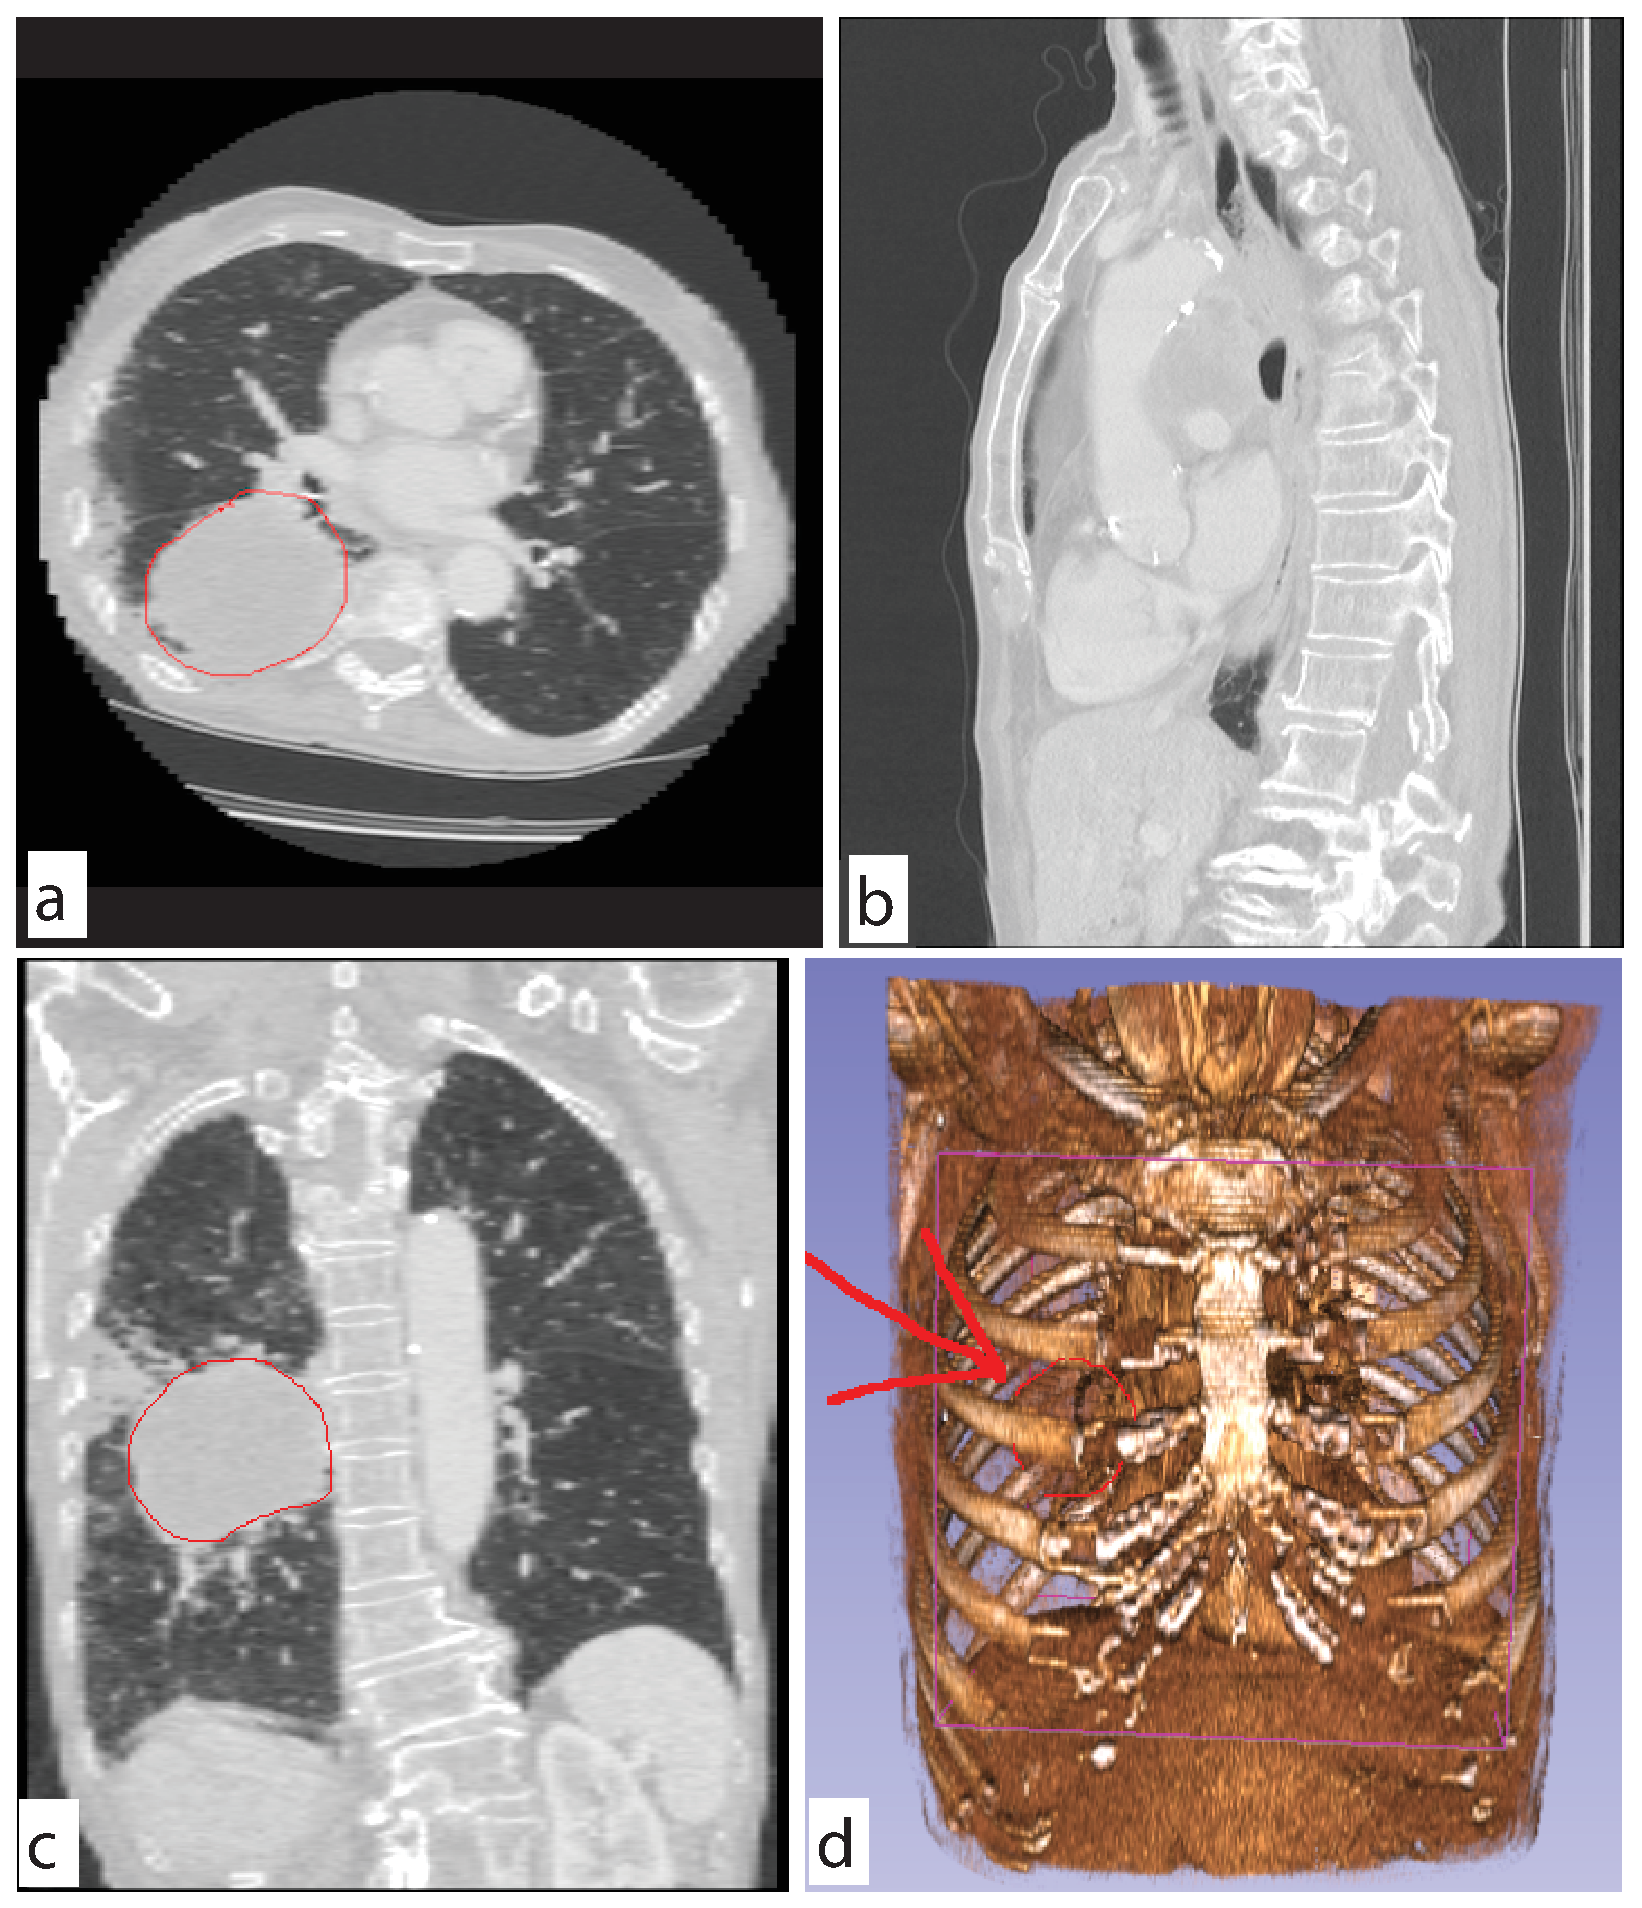
\includegraphics [width=0.48\textwidth]{images/slicer.eps}
\caption{Lung tumor visualization using slices (a-c) and standard DVR (d). Annotations are manually added by the examiner to delineate the tumor location. Images constructed using the 3D Slicer tool\,\cite{slicer}.}
\label{f:slicer}
\end{figure}

We next use our lens for this task. Sample snapshots obtained in this process are shown in \autoref{f:params}. Comparing these with standard DVR (\autoref{f:slicer}d), several points can be made. First, the tumor is significantly more visible when using the lens, both in terms of removing the occluding tissue and in terms of the tumor's opacity -- compare the inset in \autoref{f:slicer}d with the images in \autoref{f:params}. Secondly, relighting the tumor from various directions allows one to see small-scale morphological details such as the tumor's surface shape and its connection via protuberances and veins with the lung walls.

To assess the added-value of our lens, we asked the two medical specialists (pulmonologist and radiologist) involved in treating the patient that this dataset came from to study the lens' features and state its potential advantages and/or limitations as compared to standard techniques they use in their practice. Both specialists have a 10-plus year medical experience in treating lung cancer, and routinely use several slicing and DVR software tools. They work in a private hospital in Belgium, and are not actively associated to medical imaging research. Moreover, our (authors') identities were hidden from them, by using a neutral proxy communicator in the interaction. The provided input can be summarized as follows: The occlusion-free lens is definitely easier and faster to use than classical DVR and/or slicing techniques. It is especially more effective than these to get a quick, first impression of a deep buried anatomical detail. While it has several parameters, changing these by direct interaction is considerably easier to do than tuning the typical parameters of DVR to obtain similar results. This `tempts' the user to exploration, which is a good aspect. The fact that the lens minimizes viewpoint change (volume rotation), \emph{i.e.}, after a suitable viewpoint was found from which a (small) part of the target is visible, one doesn't need to change this viewpoint, is a very strong feature, as viewpoint changes are disruptive and cost time. This is especially important in a cost-aware environment where specialists have very limited time (10 minutes) to fully assess a patient examination. However, the lens cannot and should not replace classical slice-based investigation, which shows small-scale details better. This is especially important for assessing small-size lesions, tumors, or other similar anatomical features, that the lens will arguably not be able to help with, as these are too small in the first place to attract the attention of the examiner looking at a standard DVR rendering.

\begin{figure}
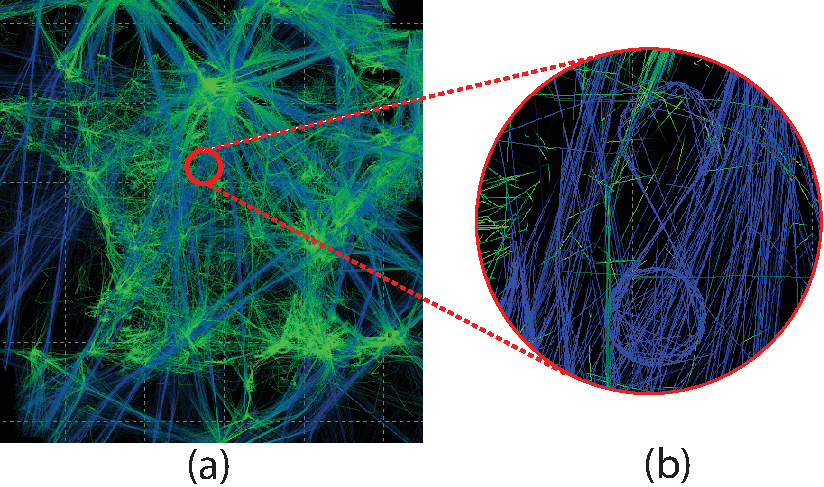
\includegraphics [width=0.45\textwidth]{images/aircraft.pdf}
\vspace{-0.15cm}
\caption{2D visualization of one day of recorded aircraft trajectories over France\,\cite{hurter2009fromdady}. (a) Overview of all trails. (b) Zoom, filtering, and color mapping techniques are used to highlight an outlier trajectory of an aircraft performing an eight-shaped loop. Revealing this outlier costs significant user effort.}
\label{f:fromdady}
\vspace{-0.15cm}
\end{figure}


\subsection{Aircraft trajectories: Outliers in the French sky}
%
%
Our final use-case considers a task from the air traffic planning field -- detecting and studying outliers in large-scale datasets containing tens of thousands of 3D (latitude, longitude, height) trails of aircraft over a given spatio-temporal region\,\cite{hurter2014interactive}. Typically, such datasets are displayed using 2D (latitude, longitude) plots where opacity encodes the spatial density of flights. \autoref{f:fromdady}-a shows one day of recorded aircraft trajectories over the French air space using this 2D technique. \autoref{f:fromdady}(b) shows a detail zoom-in of this dataset, where we can see an abnormal -- that is, not relativlyu straight -- aircraft trajectory: A tanker aircraft performed an eight-shaped loop as it was waiting to refuel other aircraft. Revealing such patterns using 2D techniques, \emph{e.g.} \cite{hurter2009fromdady}, is very hard. In particular, it is hard to de-occlude these patterns from the overall context of criss-crossing aircraft trails, even when one knows their 2D spatial location.

Our lens can help for this task, as follows. We first convert the set of 3D trails to a $500^3$ density volume, using KDE as described for the streamline use-case (Sec.~\ref{sec:flow}). Examining this volume using standard DVR allows us to see that there is an outliner (that is, not straight) trail at some point in space, see curved patterns in \autoref{f:aircraft_lens}a. By activating the lens on this area and interactively tuning the target depth $t_{min}$ (since we don't know the height of this trail), we can quickly obtain a view where the outlier trajectory is in focus and the occluding ones are pushed away (\autoref{f:aircraft_lens}a). Finally, just as in the other examples presented so far, the user can quickly change the magnification factor and view direction to better study this trajectory in context (\autoref{f:aircraft_lens}b-d). From these images, one directly and easily sees that the outlier trajectory has an eight shape. Revealing this outlier trail using standard 2D visualization techniques\,\cite{hurter2009fromdady} costs several minutes. Doing the same using our lens approach costs under one minute, for the same users. Additionally, if we compare Figs.~\ref{f:fromdady}b and~\ref{f:aircraft_lens}b-d, we argue that the eight-shape of the outlier trajectory is much more prominent, and thus recognizable, in the latter images (using our lens) than in the former ones. Last but definitely not least: The 3D volume rendering approach that our lens is based on explicitly encodes the flight height information, so our lens can use it by interactively tuning the depth value $t_{min}$ where the lens is focused. This is not possible with 2D techniques which ignore this depth dimension.
\textcolor{red}{
We validated our finding with an air traffic data scientist with more than 10 year experience. She confirmed that this specific eight shape trail is an actual aircraft which performed waiting loops and acted as a fuel supplier for military aircraft.
Compared to standard 2D visualization techniques, our system helps to detect without complex manipulation outlier trails. The user does not have to deal with color manipulation such as transparency adjustment to make this specific eight shapes emerge. As a drawback, our system creates many occlusions with opaque areas. The view is then spoiled with many artifacts which hinders the visualization of specific trails. As a solution, the user can use our lens to distort the space and locally remove occlusion. Finally, the user can modify the distortion parameters to find a suitable point of view. This example shows how our technique helps to make specific shape emerge which creates extra occlusion which is corrected thank to our obstruction free lens technique.}

 


\begin{figure*}[htbp]
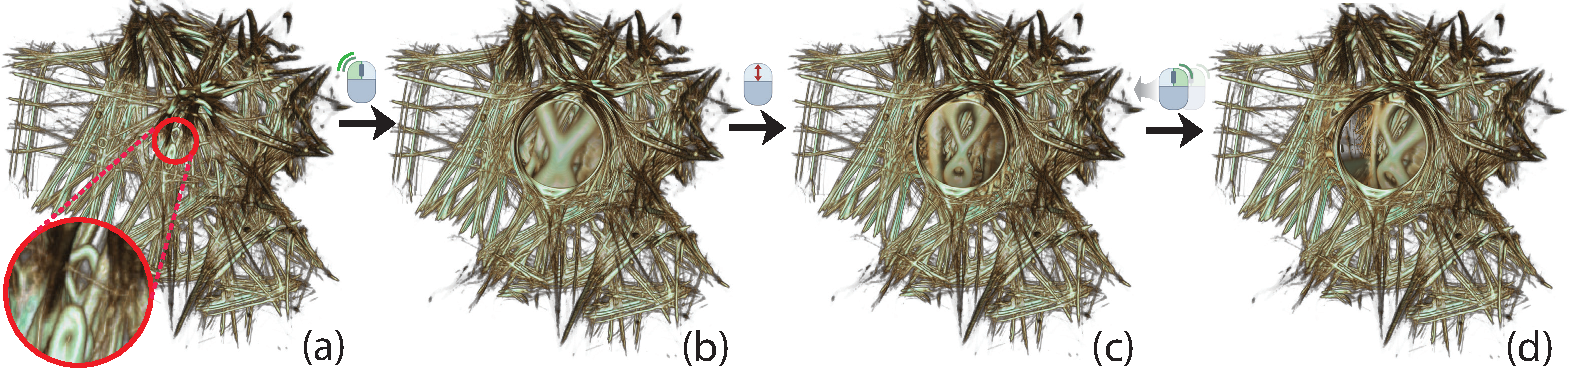
\includegraphics [width=\textwidth]{images/aircraft_lens.pdf}
\caption{Inspecting an abnormal aircraft trajectory. (a) The initial view on the trajectories where the abnormal trajectory is spotted, as it is highly curved while all other trajectories are relatively straight. Activating the lens at the location of the spotted outliner (b) and changing the magnification factor (c) reveals the trajectory's eight-shape. (d) Rotating the viewpoint provides more spatial insight on the embedding of the outlier in the surrounding trajectories.}
\label{f:aircraft_lens}
\end{figure*}
%

\begin{comment}
%ALEX: I really have no idea what this image brings to the paper, it really doesn't show anything w.r.t. the lens. Remove.

\begin{figure}
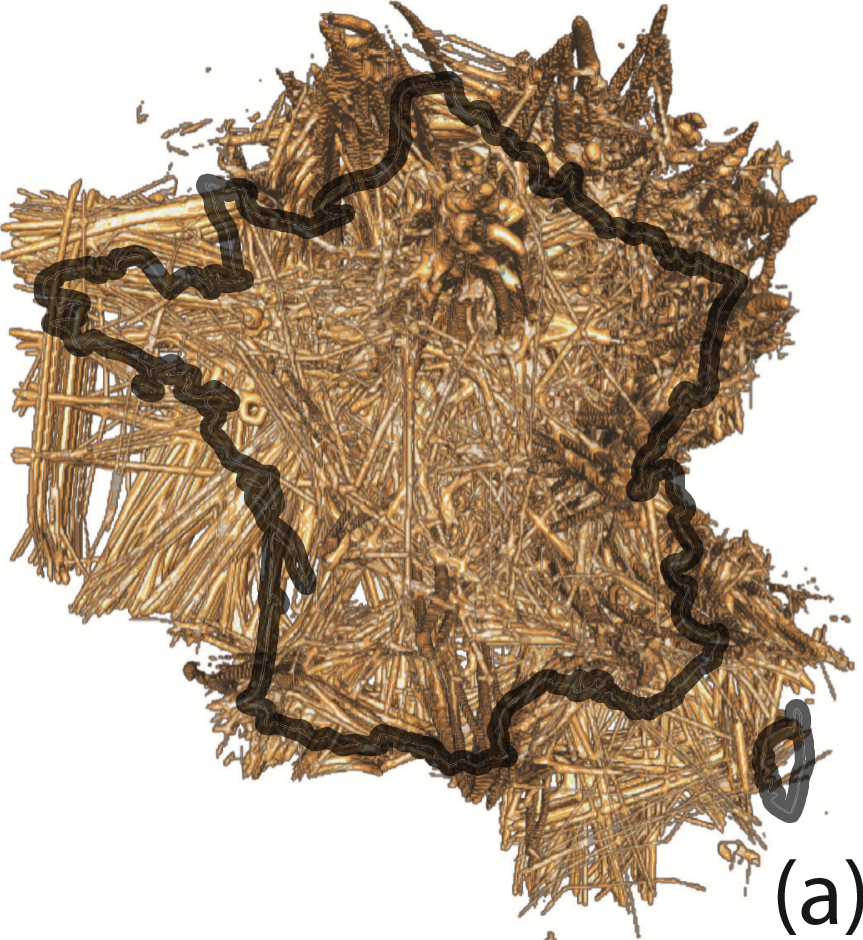
\includegraphics [width=0.36\textwidth]{images/topViewFR.png} 
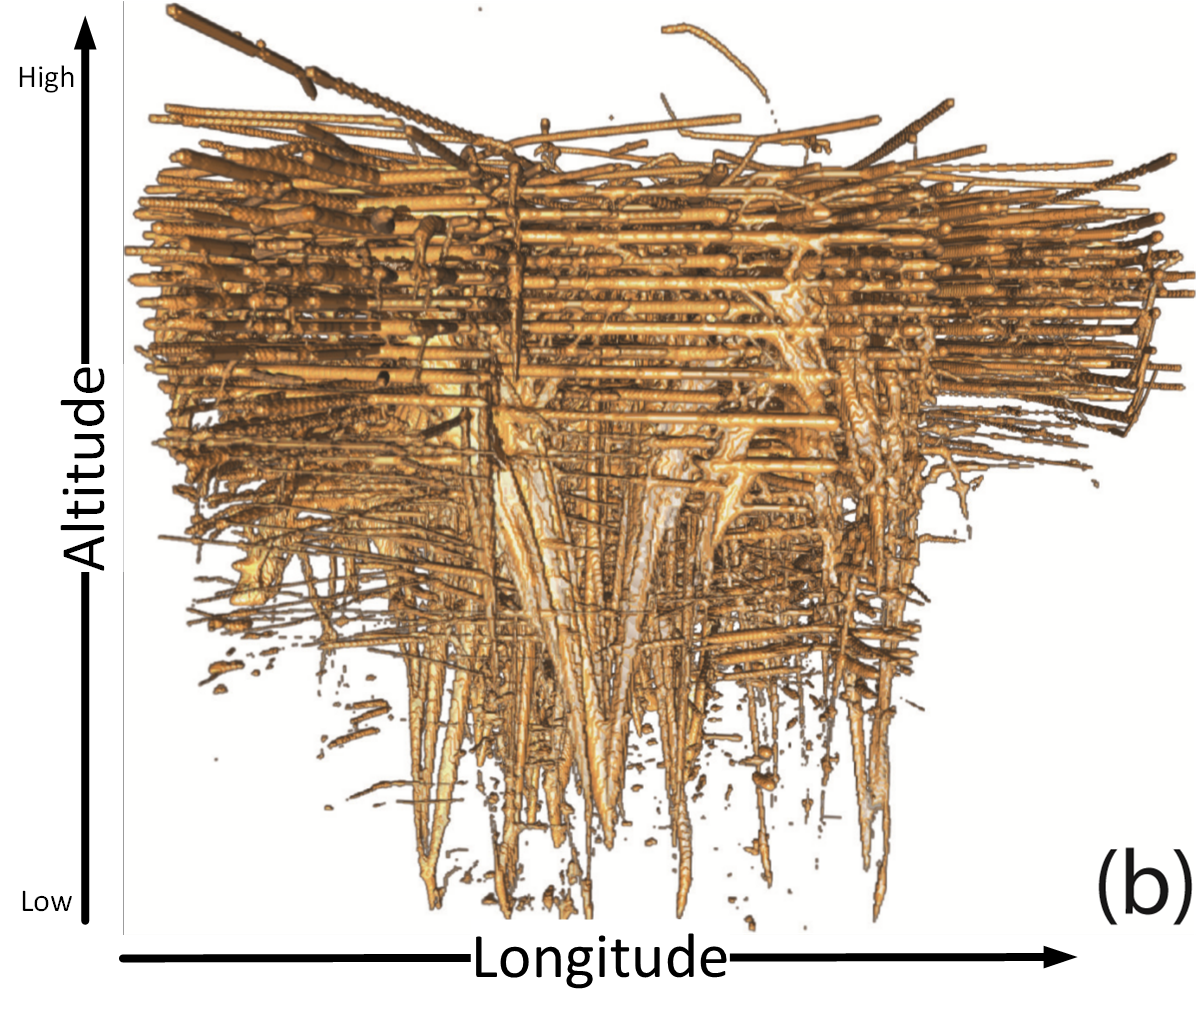
\includegraphics [width=0.4\textwidth]{images/VerticalViewLabel.png} 
\caption{Visualization of one day of recorded aircraft trajectories over France using our volume rendering framework. (a) The trajectories almost draw the map of France. (b) The trajectories are displayed according to their altitudes. }
\label{f:aircraft_orientation}
\end{figure}

\end{comment}


